\documentclass[answers,11pt]{exam}

%\documentclass[11pt]{exam}
\usepackage{enumerate}
\usepackage[utf8]{inputenc}
\usepackage{hyperref}

\usepackage{alltt}
\usepackage{xspace}
\usepackage{longtable}
\usepackage{amsfonts}
\usepackage{latexsym}
\usepackage{amsmath}
\usepackage{amssymb}
%\usepackage{xcolor}
\usepackage{enumerate}
\usepackage{graphicx}
%\usepackage{moreverb}
%\usepackage{ifthen}
\usepackage{url}
\usepackage{tikz} 
\usepackage{bussproofs}

%\usetikzlibrary{snakes}
\usetikzlibrary{decorations}
\usetikzlibrary{shapes,shapes.geometric,arrows,fit,calc,positioning,automata,decorations.pathmorphing}
\tikzset{state/.style={draw,ellipse}}

\usepackage{algorithmicx}
\usepackage[noend]{algpseudocode}
\usepackage[Algoritmo]{algorithm}


\input sli_aux
\newboolean{portuguese}
\setboolean{portuguese}{true}
\setboolean{portuguese}{false}

\newboolean{normal}
\setboolean{normal}{true}

\newcommand{\pten}[2]{\ifthenelse{\boolean{portuguese}}{#1}{#2}}
\pten{\usepackage[portuges]{babel}}{\usepackage[british]{babel}}

%\pten{\uselanguage{portuguese}}{\uselanguage{british}}

\setcounter{aula}{4}

\begin{document}
	\begin{center} 
{\bf {\large \pten{Programação Concorrente}{Concurrent Programming} - \pten{Exercícios}{Exercises} \theaula} \\

\medskip

\pten{Isomorfismo, Equivalência de Traços e Bissimulação Forte}{Ismorphism, Trace Equivalence and (Strong) Bisimulation}  }
\end{center}


\chpgword{\pten{Página}{Pages}}


\pten{Consultar os Capitulo}{Consult Chap.} 3-1-3,3 e 3.5  \pten{de}{of} \cite{aceto07:_react_system}.

\begin{questions}
\question \pten{Sendo}{Let} \begin{eqnarray*}
	P&:=& a!.0+b!.0\\
	Q&:=& b!.0+a!.0\\
\end{eqnarray*}
\pten{será que se verificam as seguintes relações}{determine if the following relations hold}
\begin{eqnarray*}
	P&\sim_{tr}&Q\\
a!.P&\sim_{tr}&a!.Q\\
a!.P+ a!.P&\sim_{tr}&a!.Q+a!.Q\\
\end{eqnarray*}
\pten{e o mesmo para}{and also for} $\sim_{iso}$?
\begin{solution}
\pten{Sim para ambas as relações.}{Yes for both relations.}
\end{solution}

\question\pten{ Mostra que}{Show}
$(b!.0+c!.0)\sim_{iso} (c!.0+b!.0)$ \pten{ mas}{but}
$a!.(b!.0+c!0)+ a!.(b!.0+c!0)\not\sim_{iso} a!.(b!.0+c!0)+ a!.(c!.0+b!.0)$
\pten{e conclui que}{and conclude that} $\sim_{iso}$ \pten{não é uma congruência}{is not a congruence}.
\question 
\pten{Mostra que para qualquer}{Show that for every} $P,Q,R\in CCS$ \begin{eqnarray*}
	P+Q &\sim_{tr}& Q+P\\
(P+Q)+R &\sim_{tr}& P+(Q+R)\\
P+0&\sim_{tr}& P,
\end{eqnarray*}	
\pten{e}{and} $\alpha.(P+Q)\sim_{tr} \alpha.P+\alpha.Q$.
\question \pten{Sendo}{Let}
\begin{eqnarray*}
	CTM&:= &coin?.(coffee!.CTM+tea!.CTM)\\
CTM'&:= &coin?.coffee!.CTM'+coin?.tea!.CTM'\\
\end{eqnarray*}
\pten{Mostra que}{Show that} $CTM \sim_{tr} CTM'$.

\question \pten{Resolver os exercícios de bissimulação  em }{Solve bisimulation problems in} \url{http://tinyurl.com/pseuco}
\question \pten{Resolver os exercícios/quizz de bissimulação (forte) em }{Solve (strong) bisimulation problems in} PseuCo Book \url{https://book.pseuco.com/#/read/equality/workout}

\question
\pten{Mostra as seguintes propriedades da relação de bissimilaridade $\sim$ }{Show that} 
\begin{parts}
\part 	$\sim$ \pten{é uma relação de equivalência}{is an equivalence relation}.
\begin{solution}
Para mostrar que é reflexiva basta mostrar que a identidade $Id=\{(P,P)\mid P\in \}$ é uma bissimulação: Se $(P,P)\in Id$ e existe $\alpha\in Act$ tal que $\trans{P}{\alpha}{P'}$ então também 
	$\trans{P}{\alpha}{P'}$ e $(P',P')\in Id$. Então $Id\subseteq \sim$ , logo $\sim$ é reflexiva.
Para a simetria, se $s_1\sim s_2$ então existe uma bissimulação $R$ tal que $(s_1,s_2)\in R$. Seja  $R^{-1}=\{(s',s)\mid (s,s')\in R\}$.  Então $(s_2,s_1)\in R^{-1}$ e $R^{-1}$ é uma bissimulação: se $\trans{s_2}{\alpha}{s_2'}$ sei que existe  $\trans{s_1}{\alpha}{s_1'}$ com $(s_1',s_2')\in R$, logo $(s_2',s_1')\in R^{-1}$. O mesmo se 
 $\trans{s_1}{\alpha}{s_1'}$. Para a transitividade seja $s_1\sim s_2$  e $s_2\sim s_3$. Temos que mostrar que $s_2\sim s_3$  Sabemos que existem duas bissimulações $R$ e $R'$ tal que $(s_1,s_2)\in R$ e $(s_2,s_3)\in R'$. Seja $$S=\{(s_1',s_3')\mid (s_1',s_2')\in R \land  (s_2',s_3')\in R'\}.$$
Temos que $(s_1,s_3)\in S$ e $S$ é uma bissimulação: se $(s,t)\in S$
então existe $w$ tal que $(s,w)\in R$ e $(w,t)\in R'$. Seja
 $\trans{s}{\alpha}{s'}$, então existe  
 $\trans{w}{\alpha}{w'}$ tal que $(s',w')\in R$ e  $\trans{t}{\alpha}{t'}$, tal que $(w',t')\in R'$. Logo $(s',t')\in S$ como queriamos. O mesmo acontece se tivermos/começarmos com $\trans{t}{\alpha}{t'}$. 
\end{solution}

\part  $\sim$ \pten{é maior bissimulação}{is the largest bisimulation}.
\begin{solution}
Por definição $\sim$ é a reunião de todas as bissimulações. Temos de mostrar que essa reunião é uma bissimulação. Pela simetria basta mostrar uma das condições. Seja $(s,t)\in \bigcup\{ R	\mid R \text{ bissimulação}\}$ e  $\trans{s}{\alpha}{s'}$. Então existe uma bissimulação $R_1$ tal que $(s,t)\in R_1$ e um $t'$ tal que $\trans{t}{\alpha}{t'}$ e $(s',t')\in R_1\subseteq  \bigcup\{ R	\mid R \text{ bissimulação}\}$. Logo $\{ R	\mid R \text{ bissimulação}\}$ é uma bissimulação.

\end{solution}

\part 	$s \sim t $ \pten{se e só se para cada}{iff for each} $\alpha\in Act$
\begin{itemize}
	\item \pten{Se}{If} $\trans{s}{\alpha}{s'}$ \pten{então existe}{then} $t'$ \pten{tal que}{such that}   $\trans{t}{\alpha}{t'}$ e $s'\sim t'$
\item  \pten{Se}{If}  $\trans{t}{\alpha}{t'}$ \pten{então existe}{then} $s'$ \pten{tal que}{such that}    $\trans{s}{\alpha}{s'}$\pten{ e }{ and} $s'\sim t'$.
\end{itemize}
\end{parts}

\question 	\pten{Seja}{Let} $TS=(S,Act,\tr)$ \pten{tal que}{such that}  $S=\{s_i\mid i\geq 1\}\cup \{t\}$, $Act=\{a\}$ e $\stackrel{a}{\tr}=\{(s_i,s_{i+1}\mid i\geq 1\}\cup \{(t,t)\}$.

\pten{Mostrar que}{Show that} $s_1\sim t$ \pten{provando que}{proving that} $R=\{(s_i,t)\mid i\geq 1\}$ \pten{é uma bissimulação}{is a bisimulation}.


\question\pten{ Considera os processos}{Let} $P$ \pten{ e }{ and} $Q$ \pten{definidos por}{be defined by}
\begin{eqnarray*}
P&:=&a.P_1+b.P_2\\
P_1&:=&c.P\\
P_2&:=&c.P
\end{eqnarray*}
\pten{ e }{ and}
\begin{eqnarray*}
Q&:=&a.Q_1+b.Q_2\\
Q_1&:=&c.Q_3\\
Q_2&:=&c.Q_3\\
Q_3&:=&a.Q_1+b.Q_2	
\end{eqnarray*}
\pten{Mostra que}{Show that} $P\sim Q$ \pten{encontrando uma bissimulação que  contenha}{presenting a bisimulation that contains} $(P,Q)$. \pten{Desenha os sistemas de transição correspondentes}{Draw their LTSs} \pten{e testa no}{and test in} pseuCo.com.

\begin{solution}
	Temos os seguintes LTSs para $P$ e $Q$, respectivamente.

\begin{tabular}{lcc}
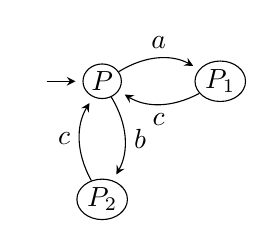
\begin{tikzpicture}[>=stealth, shorten >=2.5pt, auto, node distance=1.5cm, initial text={}]
\node[state,  inner sep=1pt, minimum size=5pt,  initial] (S0){$P$};
\node[state,  inner sep=1pt, minimum size=5pt][below of =S0] (S1){$P_2$};
\node[state,  inner sep=1pt, minimum size=5pt][right of =S0] (S2){$P_1$};
\path[->](S0) edge  [bend left] node {$a$} (S2)
(S0) edge [bend left] node {$b$} (S1)
	(S1) edge  [bend left] node {$c$} (S0)
	 (S2) edge [bend left] node {$c$} (S0);
\end{tikzpicture}&&
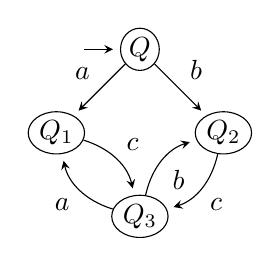
\begin{tikzpicture}[>=stealth, shorten >=2.5pt, auto, node distance=1.5cm, initial text={}]
\node[state,  inner sep=1pt, minimum size=5pt,  initial] (S0){$Q$};
\node[state,  inner sep=1pt, minimum size=5pt][below left of =S0] (S1){$Q_1$};
\node[state,  inner sep=1pt, minimum size=5pt][below right of =S0] (S2){$Q_2$};
\node[state,  inner sep=1pt, minimum size=5pt][below right of =S1] (S3){$Q_3$};

\path[->](S0) edge [swap] node  {$a$} (S1)
		edge  node  {$b$} (S2)
(S1) edge [bend left] node  {$c$} (S3)
(S3) edge [bend left] node  {$a$} (S1)
	edge [bend left,swap ] node  {$b$} (S2)
(S2) edge [bend left]node  {$c$} (S3)
;
\end{tikzpicture}
\end{tabular}
Para que $P\sim Q$ tem de existir uma bissimulação (forte) $R$ que contenha o par $(P,Q)$
A seguinte tabela mostra a construção duma bissimulação $R$. Para cada par apenas é necessário considerar as ações do primeiro elemento do par dado os LTSs serem determinísticos. As marcas $(x)$ indicam que chegamos a um par que já está em $R$ (na primeira coluna).

\begin{tabular}{l|l}
$R$& Acções\\\hline
$(P,Q)$& $\trans{P}{a}{P_1}$ e $	\trans{Q}{a}{Q_1}$\\
& $\trans{P}{b}{P_2}$ e  $	\trans{Q}{b}{Q_2}$\\\hline
$(P_1,Q_1)$& $\trans{P_1}{c}{P}$  e $\trans{Q_1}{c}{Q_2}$\\\hline
$(P_2,Q_2)$& $\trans{P_2}{c}{P}$  e $\trans{Q_2}{c}{Q_3}$ \\\hline
$(P,Q_2)$&$\trans{P}{a}{P_1}$ e $	\trans{Q}{a}{Q_1}$ (x)\\
& $\trans{P}{b}{P_2}$ e $	\trans{Q}{b}{Q_2}$ (x)\\\hline
$(P,Q_3)$&$\trans{P}{a}{P_1}$ e $	\trans{_3}{a}{Q_1}$ (x)\\
&$\trans{P}{b}{P_2}$ e $	\trans{Q_3}{a}{Q_2}$ (x)\\
\end{tabular}

Temos que a bissimulação $R=\{P,Q),(P_1,Q_1),(P_2,Q_2),(P,Q_2),(P,Q_3)\}$.

\end{solution}

\question \pten{Considera os processos}{Let} $P$ \pten{ e }{ and} $Q$ \pten{definidos por}{be defined by}
\begin{eqnarray*}
P&:=&a.P_1\\
P_1&:=&b.P+ c.P
\end{eqnarray*}
\pten{ e }{ and}
\begin{eqnarray*}
Q&:=&a.Q_1\\
Q_1&:=&b.Q_2+c.Q\\
Q_2&:=&a.Q_3\\
Q_3&:=&b.Q+c.Q_2	
\end{eqnarray*}
\pten{Mostra que}{Show that} $P\sim Q$ \pten{encontrando uma bissimulação que  contenha}{presenting a bisimulation that contains} $(P,Q)$.



\question \pten{Mostra que se}{Show that if}  $P\sim Q$ \pten{ e }{ and} $\alpha\in Act$, $R\in CCS$ \pten{ e }{ and} $H\subseteq Com$, \pten{então}{then}
\begin{eqnarray*}
	\alpha.P&\sim & \alpha.Q\\
P+R&\sim& Q+R\\
R+P&\sim& R+Q\\
P|R&\sim& Q|R\\
R|P &\sim & R|Q\\
P\backslash H &\sim &Q\backslash H
\end{eqnarray*}
	
\question \pten{Considera os processos }{ Let}
\begin{eqnarray*}
P&:=& a.(b.0+c.0)\\
Q&:=&a.b.0+a.c.0	
\end{eqnarray*}
\pten{Mostra que}{Show that} $P$ \pten{ e }{ and} $Q$ \pten{não são fortemente bissimilares}{are not strongly bisimilar}.

\begin{solution} Temos os seguintes LTSs

{\small\begin{tabular}[b]{lccr}
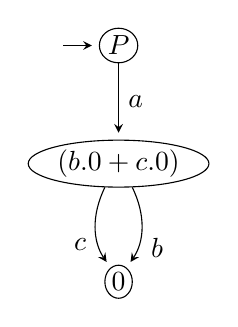
\begin{tikzpicture}[>=stealth, shorten >=2.5pt, auto, node distance=1.5cm, initial text={}]
\node[state,  inner sep=1pt, minimum size=5pt,  initial] (S0){$P$};
\node[state,  inner sep=1pt, minimum size=5pt][below of =S0] (S1){$(b.0+c.0)$};
\node[state,  inner sep=1pt, minimum size=5pt][below  of =S1] (S2){$0$};
\path[->](S0) edge  node {$a$} (S1)
	(S1) edge  [bend left] node {$b$} (S2)
	 edge  [bend right, swap] node {$c$} (S2);
\end{tikzpicture}&&
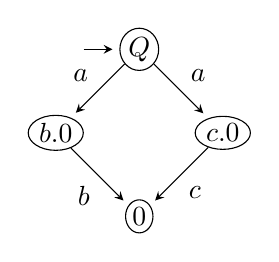
\begin{tikzpicture}[>=stealth, shorten >=2.5pt, auto, node distance=1.5cm, initial text={}]
\node[state,  inner sep=1pt, minimum size=5pt,  initial] (S0){$Q$};
\node[state,  inner sep=1pt, minimum size=5pt][below left of =S0] (S1){$b.0$};
\node[state,  inner sep=1pt, minimum size=5pt][below right of =S0] (S2){$c.0$};
\node[state,  inner sep=1pt, minimum size=5pt][below right of =S1] (S3){$0$};

\path[->](S0) edge [swap] node  {$a$} (S1)
		edge  node  {$a$} (S2)
(S1) edge [swap] node  {$b$} (S3)
(S2) edgenode  {$c$} (S3)
;
\end{tikzpicture}
\end{tabular}
}	
e os seguinte jogo de bissimulação forte enter um atacante (A), que quer mostrar que $P$ e $Q$ não são bissimilares e um defesa ($D$) que pretende mostrar que são (obtendo um bissimulação) (ver definição):
\begin{itemize}
	\item $A$: $\trans{P}{a}{(b.0+c.0)}$
\item $D$: $\trans{Q}{a}{b.0}$
\item $A$: $\trans{b.0+c.0}{c}{0}$
\item $D$ não pode jogar, logo , perde e concluímos que  $P\not\sim Q$ .
\end{itemize}

\end{solution}

\question \pten{Mostrar que}{ Show that}
\begin{eqnarray*}
		P+Q&\sim& Q+P\\
P+0&\sim& P\\
(P+Q)+R&\sim& P+(Q+R)\\
	\end{eqnarray*}
\begin{solution}
Ver Teorema 7.5 das aulas téoricas.	E também ~\cite{aceto07:_react_system}.
\end{solution}

\question \pten{Mostrar que para qualquer}{Show that for all} $P,Q,R\in CCS$,
\begin{eqnarray*}
	P|Q&\sim &Q|P\\
P|0&\sim& P\\
(P|Q)|R&\sim& P|(Q|R)\\
	\end{eqnarray*}
\pten{Nota: começa por mostrar que as seguintes relações são  bissimulações fortes:}{Show that these are bisimulations}

\begin{eqnarray*}
	&&\{(P|Q,Q|P)\mid P,Q\in CCS\},\\
	&&\{(P|0,P)\mid P\in CCS\}, \\
&&\{((P|Q)|R,P|(Q|R))\mid P,Q,R\in CCS\}.\\
\end{eqnarray*}


\question \pten{Considera a seguinte especificação de um contador}{Let}:
\begin{eqnarray*}
C_0&:= &inc. C_1\\	
 C_n&:=& inc.C_{n+1}+dec.C_{n-1}, \text{ para } n\geq 1\\
\end{eqnarray*}
\pten{e considera o processo}{and} $C:=inc.(C|dec.0)$.
\begin{parts}
\part\pten{Desenha fragmentso iniciais de}{Draw initial fragments of} 	$\bras{C}_\Gamma$ \pten{e}{and} $\bras{C_0}_\Gamma$.

\begin{solution}
\pten{Um fragmento inicial de}{A initial fragment of} $\bras{C}_\Gamma$:

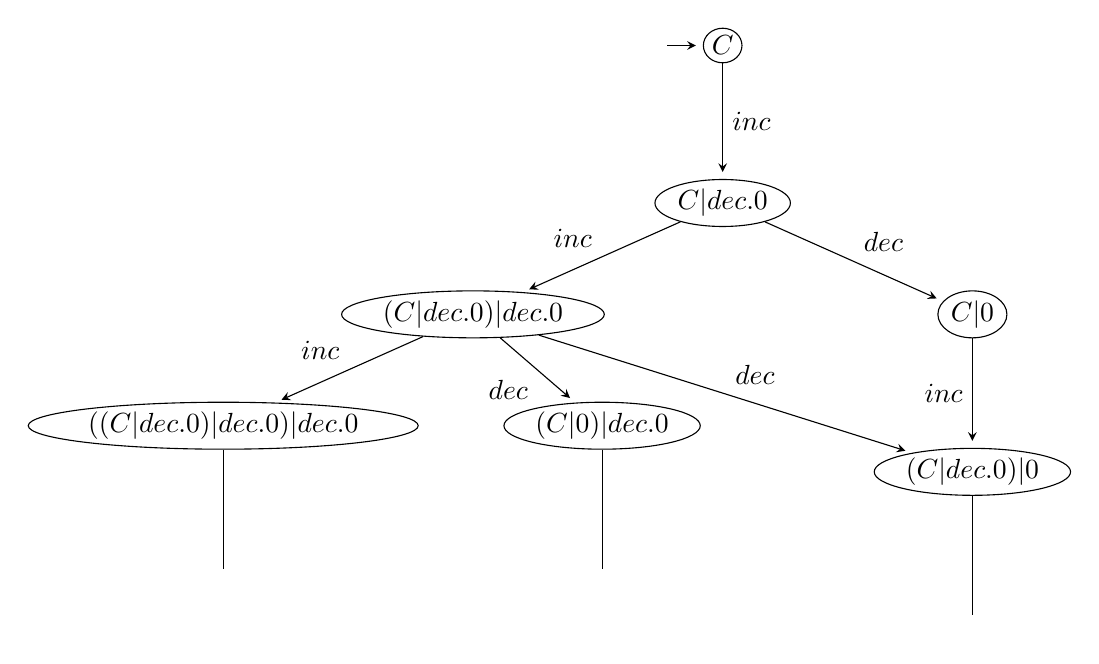
\begin{tikzpicture}[>=stealth, shorten >=2.5pt, auto, node distance=2cm, initial text={}]
\node[state,  inner sep=1pt, minimum size=5pt,  initial] (S0){$C$};
\node[state,  inner sep=1pt, minimum size=5pt][below of =S0] (S1){$C|dec.0$};
\node[state,  inner sep=1pt, minimum size=5pt, xshift=50pt][below right  of =S1] (S2){$C|0$};
\node[state,  inner sep=1pt, minimum size=5pt,xshift=-50pt][below left   of =S1] (S3){$(C|dec.0)|dec.0$};
\node[state,  inner sep=1pt, minimum size=5pt][below  of =S2] (S4){$(C|dec.0)|0$};
\node[state,  inner sep=1pt, minimum size=5pt,xshift=-50pt][below left   of =S3] (S5){$((C|dec.0)|dec.0)|dec.0$};
\node[state,  inner sep=1pt, minimum size=5pt, xshift=80pt][right   of =S5] (S6){$(C|0)|dec.0$};
\node[inner sep=1pt, minimum size=5pt][below  of =S6] (S7){};
\node[inner sep=1pt, minimum size=5pt][below  of =S5] (S8){};
\node[inner sep=1pt, minimum size=5pt][below  of =S4] (S9){};
\path[->](S0) edge  node {$inc$} (S1)
	(S1) edge  node {$dec$} (S2)
	 edge [swap]  node {$inc$} (S3)
	(S3) edge [swap]  node {$inc$} (S5)
	edge  node [swap] {$dec$} (S6)
	edge  node {$dec$} (S4)
	 (S2)  edge [swap]  node {$inc$} (S4);
\path[-] (S6) edge node {} (S7)
(S5) edge node {} (S8)
(S4) edge node {} (S9);
\end{tikzpicture}	

\pten{Um fragmento inicial de}{A initial fragment of} $\bras{C_0}_\Gamma$:
\begin{center}
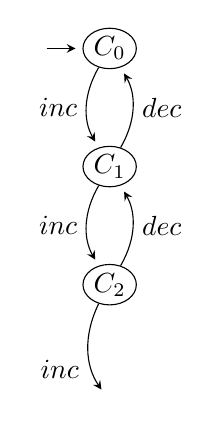
\begin{tikzpicture}[>=stealth, shorten >=2.5pt, auto, node distance=1.5cm, initial text={}]
\node[state,  inner sep=1pt, minimum size=5pt,  initial] (S0){$C_0$};
\node[state,  inner sep=1pt, minimum size=5pt][below of =S0] (S1){$C_1$};
\node[state,  inner sep=1pt, minimum size=5pt][below  of =S1] (S2){$C_2$};
\node[inner sep=1pt, minimum size=5pt][below  of =S2] (S3){};
\path[->](S0) edge [bend right, swap] node {$inc$} (S1)
	 	(S1) edge  [bend right , swap] node {$inc$} (S2)
	     edge  [bend right , swap] node {$dec$} (S0)
(S2)	 edge  [bend right, swap] node {$dec$} (S1)
		edge  [bend right , swap] node {$inc$} (S3);
\end{tikzpicture}
\end{center}
\end{solution}
\part
 \pten{Mostra que a seguinte relação é uma bissimulação}{Show that the following relation is a bisimulation}.
\begin{eqnarray*}
	\mathcal{R}&=&\{(C|\prod_{i=1}^{k}P_i,C_n)\mid k\geq 0\land  (P_i=0\lor P_i=dec.0)\\
&&\land \text{ \pten{o número de}{the number of } $i$s \pten{com}{with} $P_i=dec.0$ \pten{é}{is} $n$}\}
\end{eqnarray*}
\pten{Nota: Supõe}{Consider} $(C|\prod_{i=1}^{k}P_i,C_n)\in \mathcal{R}$. 
\

\pten{Mostra que }{Show that}
\begin{enumerate}
	\item \pten{se}{if} $\trans{C|\prod_{i=1}^{k}P_i}{\alpha}{P}$ \pten{existe}{exists} $Q$ \pten{tal que}{such that} $\trans{C_n}{\alpha}{Q}$ \pten{e}{and} $(P,Q)\in \mathcal{R}$.
\item  \pten{se}{if}   $\trans{C_n}{\alpha}{Q}$ \pten{existe}{exists} $P$ \pten{tal que}{such that} $\trans{C|\prod_{i=1}^{k}P_i}{\alpha}{P}$ \pten{e}{and}  $(P,Q)\in \mathcal{R}$.

\end{enumerate}
\end{parts}


\question \pten{Considera a especificação de um buffer com capacidade 1}{Consider a 1-Buffer}.
\begin{eqnarray*}
	B &:=& put?. get?.B
\end{eqnarray*}

\pten{Para}{For} $n\geq 1$ \pten{podemos iterativamente definir um buffer de capacidade}{we can consider a Buffer with capacity} $n$, \pten{onde}{where} $B_i^n$ \pten{indica um buffer de capacidade}{ is a buffer with capacity}  $n$ \pten{com}{with} $0\leq i\leq n$ \pten{elementos}{elements}.

\begin{eqnarray*}
	B^n_0 &:=& put?.B^n_1 \\
	B^n_i&:=& put?.B_{i+1}^n + get?.B_{i-1}^n,\;\; 0<i<n\\
	B^n_n &:=& get?.B^n_{n-1}\\
\end{eqnarray*}
\begin{parts}
\part \pten{Verifica que}{Verify that} $B\sim_{iso}B^1_0$ (\pten{desenha os seus diagramas}{draw their LTSs}).
\part \pten{Verifica que}{Verify that}  $B^2_0\sim B^1_0|B^1_0$ (\pten{desenha os seus diagramas}{draw their LTSs}).

\part \pten{Mostra que para}{Show that for} $n\geq 1$, $$  \stackrel{\scriptsize{B^n_0}\sim \underbrace{B^1_0|B^1_0|\ldots| B^1_0}}{\quad\quad n}.$$

\pten{Nota: mostrar que a seguinte relação é  uma bissimulação }{showing that the following relation is a bisimulation:}
\begin{eqnarray*}
	\mathcal{R}&=&\{(B^n_i,B^1_{i_1}|B^1_{i_2}|\ldots | B^1_{i_n})\mid i_j\in \{0,1\}\land \sum_{j=1}^{n} i_j=i\}
\end{eqnarray*}
\end{parts}

\end{questions}


\bibliographystyle{plain}      % mathematics and physical sciences
%\bibliographystyle{spphys}       % APS-like style for physics
\bibliography{bib} 


\end{document}